% AI-assisted code: generated and revised with Qwen3.8-27B
% under the author's direction; reviewed and tested by the author
% (see the thesis section "Use of AI tools").
% UML component diagram of the discovery platform (src/evoalgo, ui/src).
% Arrows point from the component that REQUIRES an interface to the one that
% PROVIDES it; the label names the interface. The dashed box is the trusted
% core (pre-built); the right column (agent backends, opencode backend, LLM provider)
% is untrusted. Only two arrows cross the trust boundary, each perpendicularly.
\documentclass[border=4pt]{standalone}
% Shared TikZ style for the thesis UML figures (standalone documents).
\usepackage[T1]{fontenc}
\usepackage{lmodern}
\usepackage{tikz}
\usetikzlibrary{positioning,arrows.meta,shapes.multipart,shapes.geometric,fit,backgrounds,calc,matrix}
\definecolor{umlfill}{HTML}{F4F6FA}
\definecolor{umlline}{HTML}{3A4150}
\definecolor{umlaccent}{HTML}{0071E3}
\tikzset{
  every node/.style={font=\sffamily\small},
  % class box: \node[class] {Name \nodepart{second} attrs \nodepart{third} ops};
  class/.style={rectangle split, rectangle split parts=3, draw=umlline, fill=umlfill,
    align=left, rectangle split part align={center,left,left}, inner sep=3pt, font=\sffamily\scriptsize},
  % generalisation (hollow triangle), realisation (dashed, hollow triangle)
  inherit/.style={-{Triangle[open,length=7pt,width=7pt]}, draw=umlline},
  realize/.style={-{Triangle[open,length=7pt,width=7pt]}, dashed, draw=umlline},
  % composition (filled diamond at the whole), aggregation (hollow), association, dependency
  compose/.style={{Diamond[length=9pt,width=6pt]}-, draw=umlline},
  aggregate/.style={{Diamond[open,length=9pt,width=6pt]}-, draw=umlline},
  assoc/.style={-, draw=umlline},
  navassoc/.style={-{Straight Barb[length=5pt]}, draw=umlline},
  depend/.style={-{Straight Barb[length=5pt]}, dashed, draw=umlline},
  mult/.style={font=\sffamily\tiny, inner sep=1pt},
  stereo/.style={font=\sffamily\tiny\itshape},
}

\begin{document}
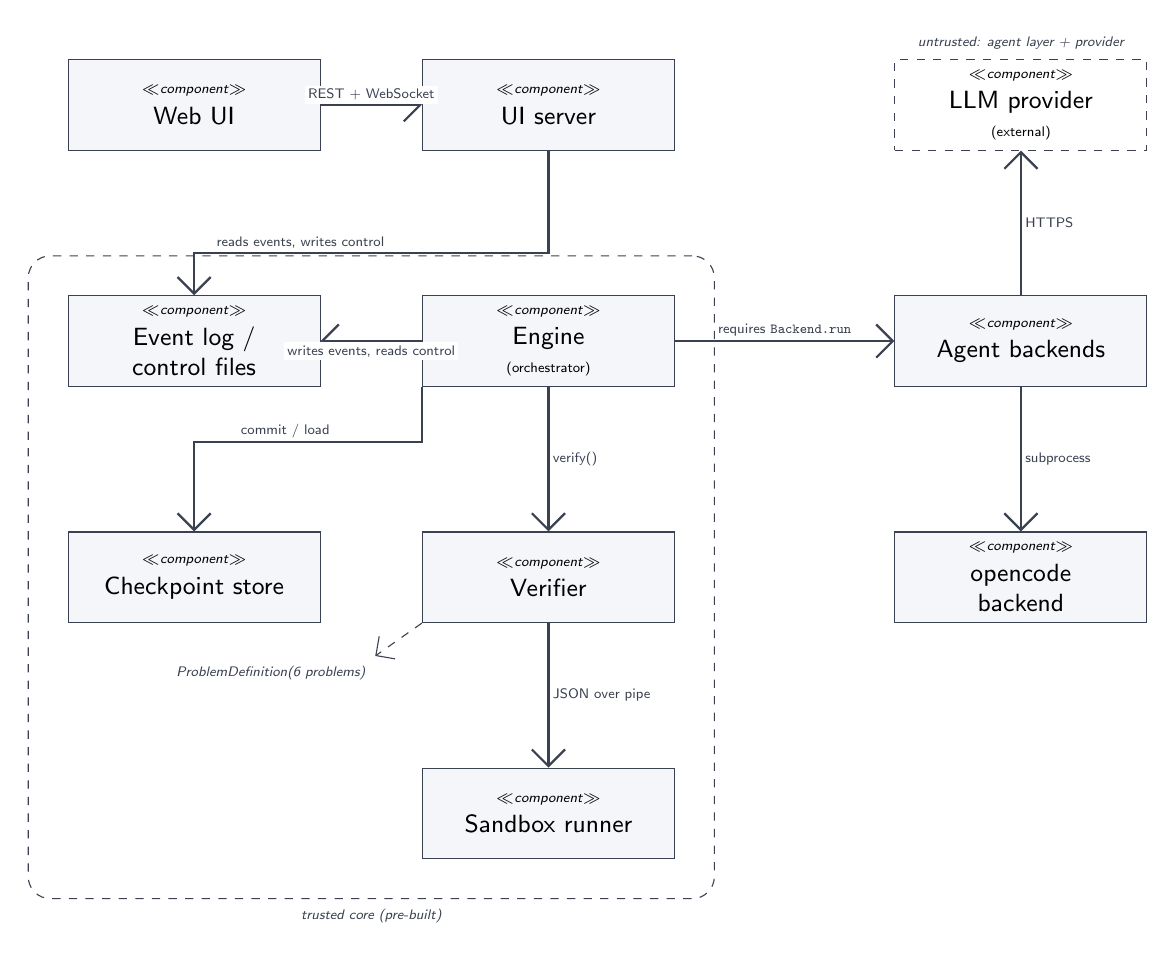
\begin{tikzpicture}[
  comp/.style={rectangle, draw=umlline, fill=umlfill, minimum width=3.2cm,
    minimum height=1.15cm, align=center, font=\sffamily\small, inner sep=2pt},
  ext/.style={comp, dashed, fill=white},
  ifc/.style={-{Straight Barb[length=6pt]}, draw=umlline, line width=0.8pt},
  ifclbl/.style={font=\sffamily\tiny, text=umlline, fill=white, inner sep=1.2pt, align=center},
  trust/.style={rectangle, draw=umlline, dashed, rounded corners=8pt, inner sep=0.5cm},
  note/.style={font=\sffamily\tiny\itshape, text=umlline},
  depend/.style={-{Straight Barb[length=5pt]}, dashed, draw=umlline},
]
  % ------------------------------------------------------------- components
  \node[comp] (ui)         at (-6,4.5)  {{\tiny\itshape$\ll$component$\gg$}\\Web UI};
  \node[comp] (server)     at (-1.5,4.5){{\tiny\itshape$\ll$component$\gg$}\\UI server};
  \node[ext]  (llm)        at (4.5,4.5) {{\tiny\itshape$\ll$component$\gg$}\\LLM provider\\[-1pt]{\tiny (external)}};
  \node[comp] (events)     at (-6,1.5)  {{\tiny\itshape$\ll$component$\gg$}\\Event log /\\control files};
  \node[comp] (engine)     at (-1.5,1.5){{\tiny\itshape$\ll$component$\gg$}\\Engine\\[-1pt]{\tiny (orchestrator)}};
  \node[comp] (backends)   at (4.5,1.5) {{\tiny\itshape$\ll$component$\gg$}\\Agent backends};
  \node[comp] (checkpoint) at (-6,-1.5) {{\tiny\itshape$\ll$component$\gg$}\\Checkpoint store};
  \node[comp] (verifier)   at (-1.5,-1.5){{\tiny\itshape$\ll$component$\gg$}\\Verifier};
  \node[comp] (harness)    at (4.5,-1.5) {{\tiny\itshape$\ll$component$\gg$}\\opencode\\backend};
  \node[comp] (sandbox)    at (-1.5,-4.5){{\tiny\itshape$\ll$component$\gg$}\\Sandbox runner};

  % --------------------------------------------------------- trust boundary
  \begin{scope}[on background layer]
    \node[trust, fit=(events)(engine)(checkpoint)(verifier)(sandbox)] (tc) {};
  \end{scope}
  \node[note, anchor=north] at (tc.south) {trusted core (pre-built)};
  \node[note, anchor=south] at (llm.north) {untrusted: agent layer + provider};

  % ------------------------------------------------------------- interfaces
  \draw[ifc] (ui.east) -- node[ifclbl, above] {REST + WebSocket} (server.west);
  \draw[ifc] (server.south) -- ++(0,-1.3) -|
        node[ifclbl, above, pos=0.35] {reads events, writes control} (events.north);
  \draw[ifc] (engine.west) -- node[ifclbl, below] {writes events, reads control} (events.east);
  \draw[ifc] (engine.south west) -- ++(0,-0.7) -|
        node[ifclbl, above, pos=0.3] {commit / load} (checkpoint.north);
  \draw[ifc] (engine.south) -- node[ifclbl, right] {verify()} (verifier.north);
  \draw[ifc] (verifier.south) -- node[ifclbl, right] {JSON over pipe} (sandbox.north);
  \draw[ifc] (engine.east) -- node[ifclbl, above] {requires \texttt{Backend.run}} (backends.west);
  \draw[ifc] (backends.north) -- node[ifclbl, right] {HTTPS} (llm.south);
  \draw[ifc] (backends.south) -- node[ifclbl, right] {subprocess} (harness.north);
  \node[note, anchor=north east] (pd) at (-3.7,-2.5) {ProblemDefinition\\[-1pt]{\tiny (6 problems)}};
  \draw[depend] (verifier.south west) -- (pd.north east);
\end{tikzpicture}
\end{document}
